%ÚVODNÍ BALÍKY, VZHLED STRÁNKY
\documentclass[aspectratio=169]{beamer} %Poměr stran 16:9, 
\usetheme{Szeged}
% Možné argumenty (doporučuji): Metropolis
% Možné argumenty (další): AnnArbor, Antibes, Bergen, Berkeley, Berlin, Boadilla, boxes, CambridgeUS, Copenhagen, Darmstadt, default, Dresden, Frankfurt, Goettingen, Hannover, Ilmenau, JuanLesPins, Luebeck, Madrid, Malmoe, Marburg, Montpellier, PaloAlto, Pittsburgh, Rochester, Singapore, Szeged, Warsaw
\usecolortheme{beaver}
% Možné argumenty: albatross, beaver, beetle, crane, dolphin, dove, fly, lily, orchid, rose, seagull, seahorse, whale, wolverine
% https://deic.uab.es/~iblanes/beamer_gallery/individual/CambridgeUS-wolverine-structuresmallcapsserif.html

\setbeamertemplate{navigation symbols}{} %Vymaže šipky na slidech
%\setbeamercovered{transparent} %Ukazuje body, které teprve přijdou zašedlé

%Zde jde odkomentovat, když chci prezentaci vytisknout na papír, např. abych si udělal poznámky tužkou. Taky jde "2 on 1" varianta.
%\usepackage{pgfpages}
%\pgfpagesuselayout{4 on 1}[a4paper, border shrink=5mm]

% Různé vychytávky
\usepackage{multicol} % Sloupce
\usepackage[shortlabels]{enumitem} % Zkrácené číslování
% Grafiky - vkládání obrázků
\usepackage[dvipsnames]{xcolor} % Barvičky
\usepackage{graphicx} % Základní
\usepackage{graphbox} % Obalování boxem zvláštních vlastností 1
\usepackage{adjustbox} % Obalování boxem zvláštních vlastností 2
% Matematické zápisy
\usepackage{mathtools} % Rozšíření asmmath - všechna matika.
\usepackage{amsfonts} % Matematické fonty
\usepackage{amssymb} % Matematické symboly
\usepackage{array}
%\usepackage[shortlabels]{enumitem}
%Balíčky s běžnými fonty a znakovými sadami
\usepackage[czech]{babel} % Čeština
\usepackage[utf8]{inputenc}   % Varianta pro unicode UTF-8
% \usepackage[latin2]{inputenc} % Varianta pro iso8859-2
% \usepackage[cp1250]{inputenc} % Varianta pro win1250

 %Vlastní příkazy
 \NewDocumentCommand{\highlight}{ +m }{\textbf{\color{ForestGreen}#1}}
 \NewDocumentCommand{\Highlight}{ +m }{\noindent\textbf{\color{ForestGreen}#1}}
 \newcommand{\predepsaneKody}[1]{}
 
 %Vlastní barvy 
 \definecolor{Gray}{gray}{0.5} 

 %Definice sloupců tabulek typu Centerer, Left a Right
 \newcolumntype{C}[1]{>{\centering\let\newline\\\arraybackslash\hspace{0pt}}m{#1}}
 \newcolumntype{L}[1]{>{\raggedright\let\newline\\\arraybackslash\hspace{0pt}}m{#1}}
 \newcolumntype{R}[1]{>{\raggedleft\let\newline\\\arraybackslash\hspace{0pt}}m{#1}}
 
 \DeclareMathOperator\tg{tg}
 \DeclareMathOperator\cotg{cotg}
 
%==================================================  Krajíčkovské úpravy  ================================================================
\usepackage{pgfplots} \pgfplotsset{compat=1.18} % ...................pgf pro grafy
\pgfplotsset{height=200pt} %velikost

\definecolor{spse}{HTML}{a32020}
\definecolor{spse2}{HTML}{b88b00}
\definecolor{akcent}{HTML}{3388cc}
\definecolor{spseIT}{HTML}{006d77}
\definecolor{spseRIS}{HTML}{ff8800}

\setbeamercolor*{palette sidebar primary}{bg=green}
\setbeamercolor*{palette primary}{use=structure,fg=white,bg=spse}
\setbeamercolor*{palette tertiary}{use=structure,fg=white,bg=spse}
\setbeamercolor*{palette quaternary}{use=structure,fg=white, bg=spse}
\setbeamercolor{title}{fg=white}

\setbeamertemplate{blocks}[default]
\setbeamertemplate{blocks}[shadow=false]
\setbeamercolor{block title}{fg=black,bg=akcent}
\setbeamercolor{block body}{fg=black, bg=akcent!40}
\setbeamercolor{block title example}{fg=black,bg=spse2}
\setbeamercolor{block body example}{fg=black, bg=spse2!40}
\setbeamercolor{block title alerted}{fg=black,bg=spse!80}
\setbeamercolor{block body alerted}{fg=black, bg=spse!40}

\usepackage{parskip}
\usepackage{xparse}

\usefonttheme[onlymath]{serif} %...........pro dobrý matematický text

\usepackage{hyperref}%.....................odkazy na web
\hypersetup{
    colorlinks=true,
    linkcolor=black,    
    urlcolor=cyan,
    }
\usepackage{multirow} %....................pro lepší tabulky..........
\renewcommand{\arraystretch}{1.5}

\usepackage{cancel} %......................pro škrtání v text
\renewcommand{\CancelColor}{\color{Red}}

\newcommand{\ablock}[2]{\begin{alertblock}{#1 \hfill \rule{0.3cm}{0.4pt} \hspace{0.02cm} $\square$ \hspace{0.02cm} \textbf{X}} #2 \end{alertblock}}
\newcommand{\eblock}[2]{\begin{exampleblock}{#1 \hfill \rule{0.3cm}{0.4pt} \hspace{0.02cm} $\square$ \hspace{0.02cm} \textbf{X}} #2 \end{exampleblock}}
\newcommand{\nblock}[2]{\begin{block}{#1 \hfill \rule{0.3cm}{0.4pt} \hspace{0.02cm} $\square$ \hspace{0.02cm} \textbf{X}} #2 \end{block}}


%===================================================== Úpravy pro TUTO prezentaci ====================================================
\newcommand{\C}{$\mathbb{C}$}
\newcommand{\R}{$\mathbb{R}$}
\setbeamercolor{button}{bg=spse}
\newcommand{\reseni}[1]{\ \hfill \hyperlink{#1}{\beamergotobutton{\Large Řešení}}}
\newcommand{\zpet}[1]{\hyperlink{#1}{\beamerreturnbutton{\Large Zpět}} \hfill }

%Vysvětlivky v rovnicích
\newcounter{mybox} %https://tex.stackexchange.com/questions/117396/how-to-put-arrows-pointing-to-equalities-to-explain-each-step
\newcommand\tikzmark[1]{%
\tikz[remember picture,overlay] \node[inner xsep=0pt] (#1) {};
}
\newcommand\ColorBox[2][]{%
\stepcounter{mybox}%
\node[draw=red!70!black,fill=red!20,align=left,#1] (box\themybox) {#2};
}

%===========================================     ÚVODNÍ SLIDE    =========================================================================
\title{Komplexní čísla}
\author{II. ročník}
\date{Poslední aktualizace: \today}
\begin{document}
\maketitle

%JÁDRO PREZENTACE
\section{Úvod}
	\begin{frame}{Jak je to s čísly...}
	 Pamatujete na čísla? Jaké druhy máme? \\[2ex]
	 $\mathbb{N}$, $\mathbb{Z}$, $\mathbb{Q}$, $\mathbb{R}$... \\[2ex]
	 Nicméně to nevypadá dosti komplexně... 
	\end{frame}
	
	\begin{frame}{Uzavřenost množin}
	Vždy vyjde číslo ze stejné množiny: \\[2ex]
	$\mathbb{N}$ - můžu napočítat předměty/ věci \\[2ex]
	$\mathbb{Z}$ - můžu libovolně odečítat čísla \\[2ex]
	$\mathbb{Q}$ - můžu libovolně dělit (vyjádřit poměr) \\[2ex]
	$\mathbb{R}$ - můžu znázornit libovolné číslo na číselné ose \\[2ex]
	\C  - ? 
	\end{frame}
		
	\begin{frame}{Co kdyby?}
	Pamatujete na kvadratickou rovnici?
		\ablock{Řešení kvadratické rovnice}{
		Kvadratická rovnice ve tvaru: $$ax^2+bx+c=0$$ má následující počet řešení: \\
			\begin{itemize}
			\item žádné řešení, jestliže $D<0$
			\item jedno řešení, jestliže $D=0$
			\item dvě řešení, jestliže $D>0$, kde $D=b^2-4ac$
			\end{itemize}}
		Co kdyby ale kvadratická rovnice měla vždy řešení? Nebylo by to super? 
	\end{frame}
	
	\begin{frame}{Definice imaginární jednotky}
		\ablock{Imaginární jednotka}{
		Imaginární jednotkou rozumíme takové "číslo" $i$, pro které platí následující vztah: $$i^2 = -1$$}
	\textbf{Doporučení:} Nepřemýšlejte, proč to tak je, jak je to možné... Je vhodné to přijmout jako fakt (prostě to tak je) a časem se vše vyjeví, proč to tak je. (Matematika je taky dospělá - o své problémy se dokáže postarat sama... \\[2ex]
	Někdy budeme též používat výše uvedenou rovnost po odmocnění: $$i=\sqrt{-1}$$ což v reálných číslech možné není (neexistuje takové číslo, kterému by se rovnala $\sqrt{1}$).
	\end{frame}
	
		\begin{frame}{Uzavřenost množin}
	Vždy vyjde číslo ze stejné množiny: \\[2ex]
	$\mathbb{N}$ - můžu napočítat předměty/ věci \\[2ex]
	$\mathbb{Z}$ - můžu libovolně odečítat čísla \\[2ex]
	$\mathbb{Q}$ - můžu libovolně dělit (vyjádřit poměr) \\[2ex]
	$\mathbb{R}$ - můžu znázornit libovolné číslo na číselné ose \\[2ex]
	\C  - můžu libovolně odmocňovat reálné číslo
	\end{frame}
	
\section{Algebraický tvar $\mathbb{C}$}

	\begin{frame}{Algebraický tvar komplexního čísla} %DOPLNIT šipečky
	\ablock{Algebraický tvar \C}{
	Je takový tvar komplexního čísla, který se zapisuje "normálně": 
		$$\tikzmark{a}a + \tikzmark{b}b \cdot \tikzmark{i}i$$}
	Není třeba se ničeho bát (imaginární číslo není reálné...) \\[2ex] 
	Imaginární jednotka zde působí jako proměnná - a v podstatě se s ní i takto pracuje
	\end{frame}
	
	\begin{frame}{Operace s komplexními čísly}
	 \eblock{Sčítání a odčítání}{
	  + a - je velice intuitivní - sečteme/odečteme zvlášť reálnou část a imaginární část:
	  $$(2+2i)+(3+i)=5+3i \hspace{3cm}(2+2i)-(3+i)=-1+i$$}
	 Závorky jsou zde pro přehlednost - sčítáme/odečítáme DVĚ komplexní čísla a výsledkem je JEDNO komplexní číslo. Běžně se závorky nepíší.
	 \eblock{Násobení}{
	  Násobení je taktéž intuitivní - roznásobíme dvě závorky::
	  $$(2+2i)\cdot(3+i)=6+6i+2i+2i^2=6+8i-2=4+8i$$
	  Nesmíme zapomenout na to, že $i^2 = -1$}
	\end{frame}
	
	\begin{frame}{Operace s komplexními čísly}
	 \eblock{Dělení}{
	 Pokud dělíme dvě komplexní čísla, zapíšeme toto dělení do zlomku. Následně zlomek "usměrníme" (místo odmocniny se zbavujeme $i$):
	 $$(-2+3i):(1+i) = \dfrac{-2+3i}{1+i} \cdot \dfrac{1-i}{1-i} = \dfrac{(-2+3i)\cdot(1-i)}{1-i^2} = \dfrac{-1+5i}{2}=-\dfrac{1}{2}+\dfrac{5}{2}i$$}
	 Podobně jako u usměrňování zlomků, využíváme vzorce $(a-b)(a+b) = a^2-b^2$. Nicméně v případu komplexních čísel, lze tento vzorec "upravit":
	 $$(a+bi)(a-bi) = a^2+b^2$$
	\end{frame}
	
	\begin{frame}[label=C1]{Cvičení - operace v algebraickém tvaru}
	\begin{tabular}{cccc}
	$(3+2i)+(2-2i)$ & $(1+2i)+2i$ & $4+(2-i)$ & $(-1+2i)+(-2+4i)$ \\
	$(3+2i)-(2-2i)$ & $(1+2i)-2i$ & $4-(2-i)$ & $(-1+2i)-(-2+4i)$ \\
	$(3+2i)\cdot(2-2i)$ & $(1+2i)\cdot 2i$ & $4\cdot (2-i)$ & $(-1+2i)\cdot (-2+4i)$ \\
	$(3+2i):(2-2i)$ & $(1+2i): 2i$ & $4:(2-i)$ & $(-1+2i):(-2+4i)$ \\[2ex]
	\end{tabular} \\
	\reseni{Ř1}
	\end{frame}
		
	\begin{frame}{Geometrické znázornění \C}
	Podobně jak reálná čísla znázorňujeme na ose reálných čísel:\\
	 \begin{tikzpicture}[>=stealth, scale=1.2]
     \draw[->] (-4,0) -- (6,0) node[right] {$x$};
     \foreach \x/\lab in {-3/ -3, 0/ 0, 1/ 1, 3.1416/ \pi, 1.4142/\sqrt{2}, 5/ 5}
        \draw (\x,0.1) -- (\x,-0.1) node[below] {$\lab$};
	 \end{tikzpicture} \\
	 \begin{minipage}{0.58\textwidth}
	Tak i \C \ mají své geometrické znázornění
	 \ablock{Gaussova rovina}{
	Gassovou rovinou rozumíme takovou rovinu, kde $x$ osa znázorňuje reálnou část komplexního čísla (značenou $\Re$), a osa $y$ znázorňuje imaginární část komplexního čísla (značenou $\Im$)}
	Body v této rovině znázorňují všechna komplexní čísla (podobně jako reálná osa znázorňuje všechny reálná čísla.
	 \end{minipage}
	 \begin{minipage}{0.4\textwidth} \hspace{4ex}
	  \begin{tikzpicture}[>=stealth, scale=1.0, font=\footnotesize]
      \draw[->] (-2.2,0) -- (2,0) node[anchor=south west] {$\Re$};
      \draw[->] (0,-2.2) -- (0,2.2) node[right] {$\Im$};
      \draw[step=1,gray!30] (-2,-2) grid (2,2);
      \foreach \x in {-2,-1,1,2}
         \draw (\x,0.1) -- (\x,-0.1) node[below] {\x};
      \foreach \y in {-2,-1,1,2}
         \draw (0.1,\y) -- (-0.1,\y) node[left] {\y $i$};
      \draw[dashed] (2,0) -- (2,1);
      \draw[dashed] (0,1) -- (2,1);
      \filldraw[red] (2,1) circle (2pt) node[above right] {$2 + i$};
	  \end{tikzpicture}
	 \end{minipage}
	\end{frame}
	
	\begin{frame}{Absolutní hodnota \C}
	Absolutní hodnotou z pohledu geometrie rozumíme vzdálenost od "počátku" (od $0$ v případě $\mathbb{R}$, v případě \C \ pak od $0+0i$) - tato definice je stejná nicméně má různé důsledky: \\
	 \begin{minipage}{0.48\textwidth}
	  \ablock{Absolutní hodnota v $\mathbb{R}$}{
	  Absolutní hodnotou $|x|$ , kde $x\in \mathbb{R}$, rozumíme číslo: \\
	  $$|x| = \begin{cases} x & \text{pro}\ x>0 \\ 0 & x=0 \\ -x & \text{pro}\ x<0 \end{cases}$$}
	 \end{minipage} 
	 \begin{minipage}{0.48\textwidth}
	  \ablock{Absolutní hodnota v \C}{
	   Absolutní hodnotou $|z|=|a+bi|$, kde $a,b \in \mathbb{R}$, rozumíme \textbf{reálné} číslo: $$|z|=|a+bi|=\sqrt{a^2+b^2}$$}
	 \end{minipage}
	\end{frame}
	
	\begin{frame}{Číslo opačné a sdružené}
	 \ablock{Číslo opačné}{
	 	\begin{minipage}{0.6\textwidth}
	 	 Číslo opačné k číslu $x$ se rozumí číslo $-x$. Stejně tak v komplexních číslech: číslo opačné k číslu $2+i$ je číslo $-(2+i) = -2-i$.
	 	\end{minipage} \hspace{4ex}
		\begin{minipage}{0.3\textwidth}
				  \begin{tikzpicture}[scale=0.8, font=\footnotesize]
				     \draw[step=1,gray!30] (-2,-1) grid (2,1);
     				 \draw[->, thick] (-2.2,0) -- (2.2,0) node[anchor=south west] {$\Re$};
     				 \draw[->, thick] (0,-1.2) -- (0,1.2) node[right] {$\Im$};
      					\foreach \x in {-2,-1,1,2}
        				 \draw (\x,0.1) -- (\x,-0.1) node[below] {\x};
      					\foreach \y in {-1,1}
       					  \draw (0.1,\y) -- (-0.1,\y) node[left] {\y $i$};
     					 \draw[dashed, spse] (-2,-1) -- (2,1);
      					\filldraw[spse] (2,1) circle (2pt) node[right] {$2 + i$};
      					\filldraw[spse] (-2,-1) circle (2pt) node[left] {$-(2 + i)$};
	 				 \end{tikzpicture}
		\end{minipage} }
	 \ablock{Číslo komplexně sdružené}{
	 \begin{minipage}{0.6\textwidth} 
	 	 Číslo komplexně sdružené k číslu $a+bi$ se rozumí číslo $a-bi$. Značíme jej $\overline{z}$. Například když $z=2+i$, pak $\overline{z}=2-i$.
	 	\end{minipage} \hspace{4ex}
		\begin{minipage}{0.3\textwidth}
				  \begin{tikzpicture}[scale=0.8, font=\footnotesize]
				      \draw[step=1,gray!30] (-2,-1) grid (2,1);
     				 \draw[->, thick] (-2.2,0) -- (2.2,0) node[anchor=south west] {$\Re$};
     				 \draw[->, thick] (0,-1.2) -- (0,1.2) node[right] {$\Im$};
      					\foreach \x in {-2,-1,1,2}
        				 \draw (\x,0.1) -- (\x,-0.1) node[below] {\x};
      					\foreach \y in {-1,1}
       					  \draw (0.1,\y) -- (-0.1,\y) node[left] {\y $i$};
     					 \draw[dashed, spse] (2,-1) -- (2,1);
      					\filldraw[spse] (2,1) circle (2pt) node[right] {$2 + i$};
      					\filldraw[spse] (2,-1) circle (2pt) node[right] {$2 - i$};
	 				 \end{tikzpicture}
		\end{minipage} }
	\end{frame}
	
 \begin{frame}[label=C2]{Cvičení - absolutní hodnota \C}
	Určete absolutní hodnotu čísel: \\
	\begin{tabular}{cccccccc}
	$|1-i|$ & $|1+i|$ & $\left|\frac{1}{2}-\frac{\sqrt{3}}{2}i\right|$ & $|2-3i|$ & $|\sqrt{3}+i|$ & $|2-2i|$ & $|1+2i|$ & $|-2+i|$\\
	$|1+2i|$ & $|2-3i|$ & $|4-3i|$ & $|2+i|$ & $|2+i|$ & $|3+2i|$ & $|2i|$ & $|-8|$ \\
	\end{tabular} \\[2ex]
	Určete číslo komplexně sdružené: 
	\begin{tabular}{cccccccc}
	$1-i$ & $1+i$ & $\frac{1}{2}-\frac{\sqrt{3}}{2}i$ & $2-3i$ & $2+i$ & $3+2i$ & $2i$ & $-8$ \\
	\end{tabular} \\[2ex]
	Určete číslo opačné: \\
	\begin{tabular}{cccccccc}
	$1-i$ & $1+i$ & $\frac{1}{2}-\frac{\sqrt{3}}{2}i$ & $2-3i$ & $2+i$ & $3+2i$ & $2i$ & $-8$ \\
	\end{tabular} \\
	\reseni{Ř2}
	\end{frame}
	
	\begin{frame}{Zajímavé počítáníčko}
	 \begin{minipage}{0.5\textwidth}
	  \begin{tabular}{cc}
	  \textbf{Vypočítejte:} & \textbf{Určete:} \\
	   $(1+i)(1-i)$ & $|1+i|$ \\
	   $(3+4i)(3-4i)$ & $|3-4i|$ \\
	   $(\sqrt{2}+\sqrt{2}i)(\sqrt{2}-\sqrt{2}i)$ & $|\sqrt{2}+i\sqrt{2}|$ 
	  \end{tabular}
	 \end{minipage} \vspace{4ex}
	 \begin{minipage}{0.42\textwidth}
	  \begin{alertblock}{Vzorec $(a+b)(a-b)$ v \C}
	  Všimněme si, že tyto úlohy jsou si podobné. Je vhodné mít proto v paměti následující zkratku: $$z\overline{z}=(a+bi)(a-bi)=a^2+b^2$$ 
	  \end{alertblock}
	 \end{minipage}
	 \begin{alertblock}{Zajímavé vztahy}
	 Platí následující rovnosti: $$|z|=\sqrt{z\overline{z}}=\sqrt{a^2+b^2}$$
	 \end{alertblock}
	\end{frame}
	
	\begin{frame}{Geometrie sčítání a násobení}
	Podobně, jako u sčítání v $\mathbb{R}$ ($2+3=5$): \\ 
	 \begin{tikzpicture}[>=stealth, scale=1.1]
     \draw[->] (-1,0) -- (6,0) node[right] {$\mathbb{R}$};
     \draw (0,0) node[below] {$0$};
     \draw (2,-0.1) node[below] {$2$} -- (2,0.1);
     \draw (5,-0.1) node[below] {$5$} -- (5,0.1);
     \draw[->, thick, blue] (0,0.2) -- (2,0.2) node[midway, above] {$2$};
     \draw[->, thick, red] (2,0.2) -- (5,0.2) node[midway, above] {$3$};
	 \end{tikzpicture} \\[2ex]
	 \begin{minipage}{0.48\textwidth}
	 	si lze představit i sčítání v \C \ ($1+2i+3+i$): \\
	  \begin{tikzpicture}[>=stealth, scale=1.2]
	   \draw[step=0.5,gray!30] (-0.5,-0.5) grid (2.5,2);
       \draw[->] (-0.5,0) -- (2.2,0) node[right] {$\Re$};
       \draw[->] (0,-0.5) -- (0,1.8) node[above] {$\Im$};
       \draw[thick, red] (0,0) -- (0.5,1) node[above] {$1+2i$};
       \draw[thick, blue] (0,0) -- (1.5,0.5) node[right] {$3+i$};
       \draw[dashed, red] (1.5,0.5) -- (2,1.5);
       \draw[purple] (0,0) -- (2,1.5) node[above] {$4+3i$};
      \end{tikzpicture}
	 \end{minipage} \vspace{0.8cm} \hspace{1cm}
	 	 \begin{minipage}{0.4\textwidth}
	 	 i odčítání v \C \ ($1+2i-(3+2i)$): \\
	  \begin{tikzpicture}[>=stealth, scale=1.2]
	   \draw[step=0.5,gray!30] (-0.5,-0.5) grid (2.5,2);
       \draw[->] (-0.5,0) -- (2.2,0) node[right] {$\Re$};
       \draw[->] (0,-0.5) -- (0,1.8) node[above] {$\Im$};
       \draw[thick, red] (0,0) -- (0.5,1) node[above] {$1+2i$};
       \draw[thick, blue] (0,0) -- (1.5,1) node[right] {$3+2i$};
       \draw[dashed, red] (1.5,1) -- (1,0);
       \draw[purple] (0,0) -- (1,0) node[anchor=north]{$2$};
      \end{tikzpicture}
	 \end{minipage}
	 \end{frame}
	 
	 \begin{frame}{Geometrie násobení}
	  Pro $\mathbb{R}$ je interpretace jednoduchá : \\[2ex]
      \begin{tikzpicture}[scale=0.6]
        \draw[->] (-1,0) -- (7,0) node[right] {$\mathbb R$};
        \foreach \x in {0,2,4,6}
         \draw (\x,0.1) -- (\x,-0.1) node[below] {\x};
        \draw[->, thick, blue] (0,0) -- (2,0) node[midway, above] {$2$};
        \draw[->, thick, red] (0,0.05) -- (6,0.05) node[midway, above] {$2\cdot 3$};
      \end{tikzpicture}
       \hspace{1cm}
    % ====== Reálná, záporné ======
      \begin{tikzpicture}[scale=0.6]
        \draw[->] (-7,0) -- (3,0) node[right] {$\mathbb R$};
        \foreach \x in {-6,-4,-2,0,2}
         \draw (\x,0.1) -- (\x,-0.1) node[below] {\x};
        \draw[->, thick, blue] (0,0) -- (2,0) node[midway, above] {$2$};
        \draw[->, thick, red] (0,0.05) -- (-6,0.02) node[midway, above] {$(-3)\cdot2$};
      \end{tikzpicture} \\
      Pro \C \ je interpretace poněkud nejednoduchá - ukážeme se jí zatím pouze na násobení $i$:
      \begin{tikzpicture}[scale=0.8, font=\small]
        \draw[->] (-1.3,0) -- (1.3,0) node[above] {$\Re$};
        \draw[->] (0,-1.3) -- (0,1.5) node[right] {$\Im$};
        \foreach \x in {-1,1}
         \draw (\x,0.1) -- (\x,-0.1) node[below] {$\x$};
         \draw (-0.1,1) -- (0.1,1) node[right] {$i$};
         \draw (-0.1,-1) -- (0.1,-1) node[right] {$-i$};
        \filldraw[BrickRed] (1,0) circle (2pt);
      \end{tikzpicture}
	 \end{frame}


	
\section{Goniometrický tvar \C}

	\begin{frame}{Typy soustav souřadnic}
	 \begin{minipage}{0.65\textwidth}
	  	\textbf{Kartézská soustava souřadnic:}
 	  \begin{itemize}[- ]
 	   \item Osy jsou na sebe kolmé
 	   \item Máme jednotnou vzdálenost
 	  \end{itemize}
 	  Na tento systém jsme zvyklí - jak moc se posunu ve směru $x$ a $y$, abych se dostal do bodu? \\[2ex]
 	  \textbf{Polární soustava souřadnic:}
	  \begin{itemize}[- ]
 	   \item Osa je jen jedna (osa $x$)
 	   \item Je zavedený úhel
 	  \end{itemize}
 	  I když máme jednu osu pomůžeme si snadno - a to pomocí \textbf{úhlu} a \textbf{vzdálenost} - jdeme jakoby "zkratkou"
	 \end{minipage} \hspace{4ex}
	 \begin{minipage}{0.28\textwidth}
	  \begin{tikzpicture}[scale=0.3, >=stealth, font=\small]
	    \draw[step=1,color=gray!20] (-5,-3) grid (5,3);
 		\draw[->] (-5.3,0) -- (5.3,0) node[above] {$\Re$};
		\draw[->] (0,-3) -- (0,3) node[right] {$\Im$};
	  \end{tikzpicture} 
	  \begin{tikzpicture}[scale=0.3, >=stealth, font=\small]
		% Kružnice (pomocné)
		\foreach \r in {1,3,5}
 		 \draw[gray!30] (0,0) circle (\r);
		% Paprsky (tabulkové úhly)
		\foreach \a in {0,30,...,330}
 		 \draw[gray!20] (0,0) -- (\a:5.3);
 		% Osy
 		\draw[->] (-5.3,0) -- (5.3,0) node[above] {$\Re$};
		\draw[->] (0,-5.3) -- (0,5.3) node[right] {$\Im$};
 	  \end{tikzpicture}
	 \end{minipage}
	\end{frame}
	
	\begin{frame}{Příklady systému souřadnic}
	 \begin{minipage}{0.48\textwidth}
	  \textbf{Kartézský systém} \\[2ex]
 	  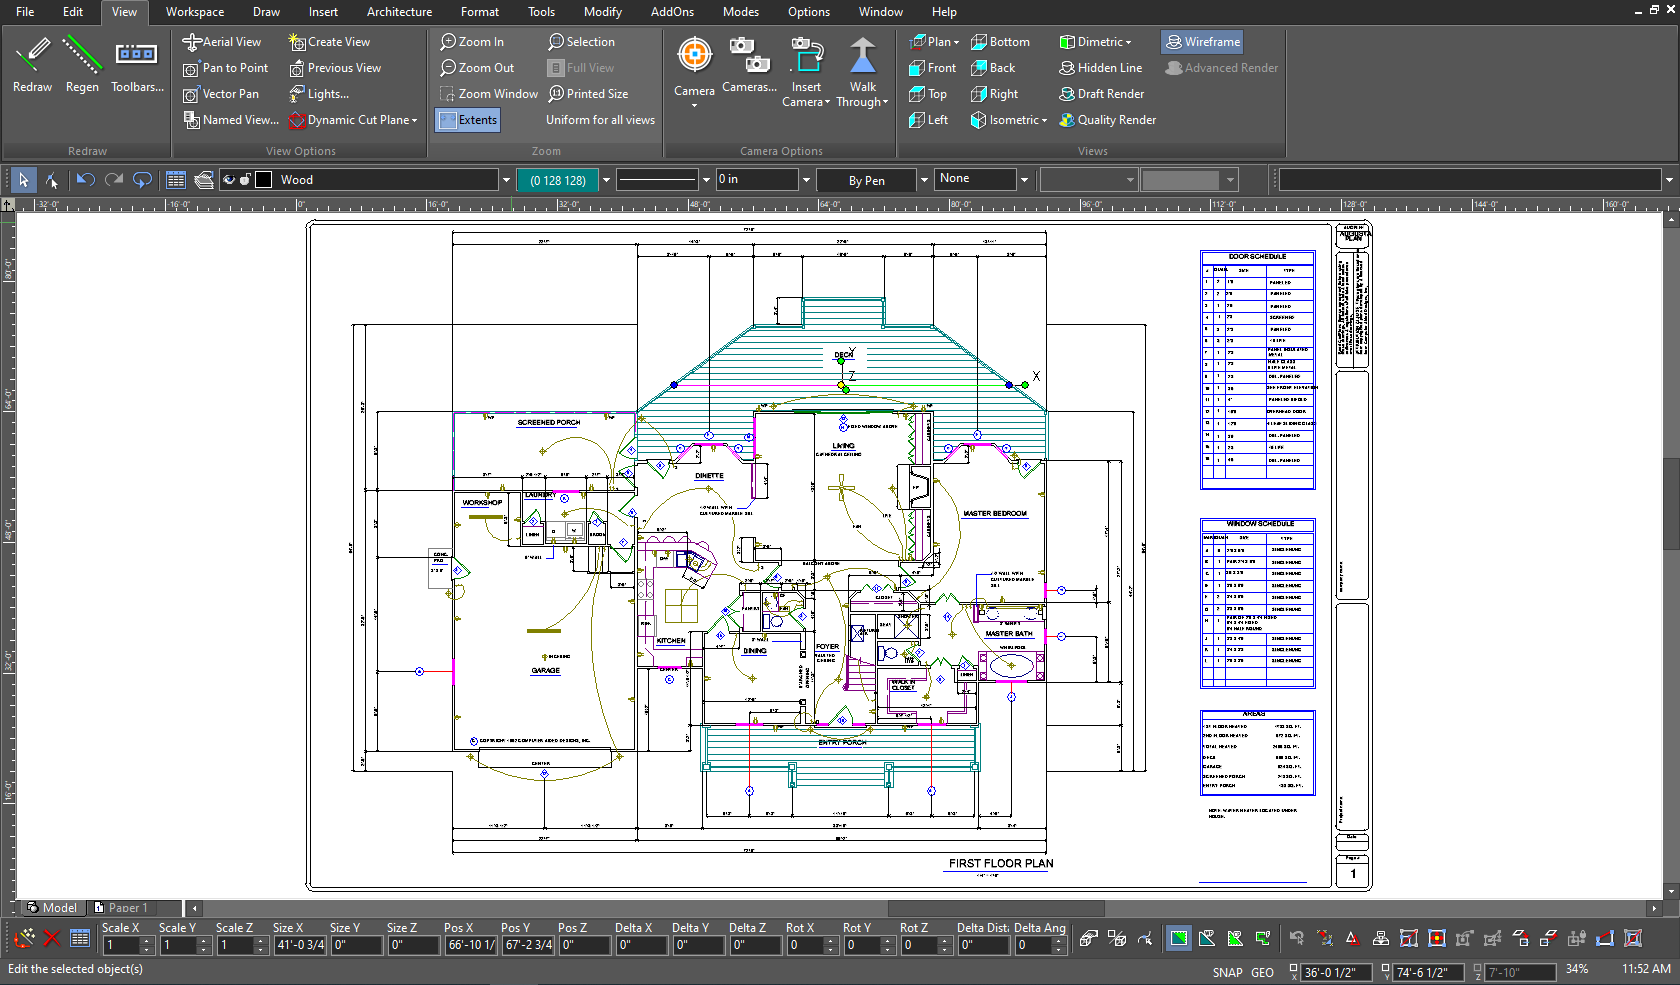
\includegraphics[scale=0.15]{Turbocad}
	 \end{minipage}
	 \begin{minipage}{0.48\textwidth}
	  \textbf{Polární systém}\\[2ex]
	  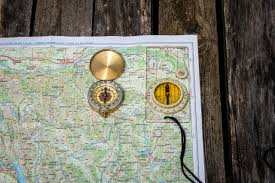
\includegraphics[scale=0.6]{mapa}
	 \end{minipage}
	\end{frame}
	
	\begin{frame}{Goniometrický tvar}
	 \begin{alertblock}{Goniometrický tvar čísla}
	 \begin{minipage}{0.5\textwidth}
	 	 Goniometrickým tvarem komplexního čísla rozumíme zápis v polárním systému souřadnic: $$z = |z|(\cos \varphi +i\sin \varphi)$$kde $|z|$ je absolutní hodnota komplexního čísla a $\varphi$ je úhel, který svírá komplexní číslo s osou $x$. 
	 \end{minipage} \hspace{4ex}
	 \begin{minipage}{0.4\textwidth}
		\begin{tikzpicture}[scale=2, >=stealth, font=\small]
    	 \draw[->] (-0.2,0) -- (1.3,0) node[above] {$\Re$};
   		 \draw[->] (0,-0.2) -- (0,1.3) node[right] {$\Im$};
	     \draw[->, thick, BrickRed] (0,0) -- (1,1) node[above] {$z$} node[pos=0.5, above, sloped]{$|z|$};
	     \filldraw[BrickRed] (1,1) circle (0.6pt);
	     \draw[thick] (0.4,0) arc (0:45:0.4);
    	 \draw (0.55,0.15) node {$\varphi$};
		\end{tikzpicture}
	 \end{minipage}
	 \end{alertblock}
	\end{frame}
	
	\begin{frame}{Goniometrický tvar}
	 \begin{minipage}{0.4\textwidth}
	 V Gaussově rovině zobrazte následující čísla:\\
	  \begin{itemize}
	   \item[\textcolor{BrickRed}{$z_1  =$}] $2(\cos 60^\circ + i\sin 60^\circ)$ \\[2ex]
	   \item[\textcolor{RoyalBlue}{$z_2  =$}] $3(\cos 150^\circ + i\sin 150^\circ)$ \\[2ex]
	   \item[\textcolor{ForestGreen}{$z_3  =$}] $\sqrt{2}(\cos 270^\circ + i\sin 270^\circ)$ \\[2ex]
	   \item[\textcolor{Orange}{$z_4  =$}] $2(\cos 315^\circ + i\sin 315^\circ)$
	  \end{itemize}
	 \end{minipage} \hspace{4ex}
	 \begin{minipage}{0.5\textwidth}
	  \begin{tikzpicture}[scale=1, >=stealth, font=\small]
	    \draw[->] (-2.2,0) -- (2.2,0) node[right] {$\Re$};
	    \draw[->] (0,-2.2) -- (0,2.2) node[above] {$\Im$};
	    % z1
	    \draw[->, thick, BrickRed] (0,0) -- (1,1.73)
         node[right] {$z_1$} node[pos=0.5,above, sloped]{2};
 	    % z2
 	    \draw[->, thick, RoyalBlue] (0,0) -- (-2.6,1.5)
         node[above] {$z_2$} node[pos=0.5,above, sloped]{3};
  	    % z3
  	    \draw[->, thick, ForestGreen] (0,0) -- (0,-1.41)
         node[right] {$z_3$} node[pos=0.5,left]{$\sqrt{2}$};
	    % z4
 	     \draw[->, thick, Orange] (0,0) -- (1.41,-1.41)
          node[right] {$z_4$} node[pos=0.5,above, sloped]{2};

	  \end{tikzpicture}
	 \end{minipage}
	\end{frame}
	
	\begin{frame}{Převod na Goniometrický tvar}
	Jak převést číslo $-1+i$ na Goniometrický tvar? Využijeme znalosti goniometrie:
	 \begin{alertblock}{Převod ALG. tvaru na GONIO. tvar}
	  \begin{minipage}{0.6\textwidth}
	   \begin{enumerate}[i) ]
	   \item Nejprve určíme $|z|$
	   $$|-1+i| = \sqrt{(-1)^2+1^2} = \sqrt{2}$$
	   \item Následně určíme úhel $\varphi$ \\
	    \begin{tabular}{C{3cm} C{3cm}}
	    $\cos \varphi = \frac{a}{|z|}$ & $\sin \varphi = \frac{b}{|z|}$ \\
	    $\cos \varphi = \frac{-1}{\sqrt{2}}$ & $\sin \varphi = \frac{1}{\sqrt{2}}$ \\
	    $\varphi = \frac{3\pi}{4}; \frac{5\pi}{4}$ & $\varphi = \frac{\pi}{4}; \frac{3\pi}{4}$ \\
	    \end{tabular}
	   \end{enumerate}
	  \end{minipage} \hspace{5ex}
	  \begin{minipage}{0.32\textwidth}
	   \begin{tikzpicture}[scale=2, >=stealth, font=\small]
    	 \draw[->] (-0.2,0) -- (1.3,0) node[above] {$\Re$};
   		 \draw[->] (0,-0.2) -- (0,1.3) node[right] {$\Im$};
   		 \draw[dashed, gray] (1,0) -- (1,1) node[pos=0.5,right]{$b$};
	     \draw[->, thick, BrickRed] (0,0) -- (1,1) node[above] {$z$} node[pos=0.5, above, sloped]{$|z|$};
	     \filldraw[BrickRed] (1,1) circle (0.6pt);
	     \draw[thick] (0.4,0) arc (0:45:0.4) node[pos=0.5, right] {$\varphi$};
	     \draw[<->, gray]  (0.05,-0.08) -- (1,-0.08) node[midway, anchor=north]{$a$};
    	\end{tikzpicture}
	  \end{minipage}
	  A teď to dáme dohromady: $z=\sqrt{2}(\cos\frac{3\pi}{4}+i\sin\frac{3\pi}{4})$
	 \end{alertblock}
	\end{frame}		
	
	\begin{frame}[label=C3]{Cvičení - převod na goniometrický tvar}
	 \begin{tabular}{cccc}
	 $1-i$ & $-5+5i$ & $3\sqrt{2}+3i\sqrt{2}$ & $\pi i$ \\ [2ex]
	 $-\dfrac{\sqrt{2}}{2}-\dfrac{\sqrt{2}}{2}i$ & $2-2i$ & $-1+i\sqrt{3}$ & $2\sqrt{3}+2i$ \\[2ex]
	 \reseni{Ř3}
	 \end{tabular}
	\end{frame}
	
	\begin{frame}{Převod na Algebraický tvar}
	 Jak převést číslo zpátky do algebraického tvaru? Zcela jednoduše - vypočítáme ho:
	 \begin{alertblock}{Převod z GONIO. tvaru na ALG. tvar}
	  Máme číslo: $z=\sqrt{2}(\cos\frac{3\pi}{4}+i\sin\frac{3\pi}{4})$\\[2ex]
	  V tomto převodu pouze číslo "spočítáme": \\[2ex]
	  $$\sqrt{2}\left(\cos\dfrac{3\pi}{4}+i\sin\dfrac{3\pi}{4}\right) = \sqrt{2}\left(-\dfrac{\sqrt{2}}{2}+i\dfrac{\sqrt{2}}{2}\right) = -1+i$$ \\[2ex] Tedy $\sqrt{2}(\cos\frac{3\pi}{4}+i\sin\frac{3\pi}{4}) = -1+i$
	 \end{alertblock}
	\end{frame}
	
	\begin{frame}[label=C4]{Cvičení - převod na algebraický tvar}
	
	\reseni{Ř4}
	\end{frame}
	
	\begin{frame}{Počítání v goniometrickém tvaru}
	Operace v goniometrickém tvaru lze znázornit (a představit si) v geometrii: 
 	 \begin{alertblock}{Sčítání a odčítání}
 	  Je lepší (a taky bezpečnější) když si čísla převedete do ALG tvaru
 	 \end{alertblock}	
 	 \begin{alertblock}{Násobení}
 	 Vynásobíme velikosti a sečteme úhly - násobení je "otáčení" \\
 	 $\sqrt{2}\left(\cos \dfrac{\pi}{3} + i\sin \dfrac{\pi}{3}\right)\cdot \sqrt{3}\left(\cos \dfrac{\pi}{6} + i\sin \dfrac{\pi}{6}\right) = \sqrt{6}\left(\cos \dfrac{\pi}{2} + i\sin \dfrac{\pi}{2}\right)$
 	 \end{alertblock}
 	 \begin{alertblock}{Dělení}
 	 Vydělíme velikosti a odečteme úhly - dělení je "opačné otáčení" \\
 	 $\sqrt{2}\left(\cos \dfrac{\pi}{3} + i\sin \dfrac{\pi}{3}\right):\sqrt{3}\left(\cos \dfrac{\pi}{6} + i\sin \dfrac{\pi}{6}\right) = \dfrac{\sqrt{2}}{\sqrt{3}}\left(\cos \dfrac{\pi}{6} + i\sin \dfrac{\pi}{6}\right)$
 	 \end{alertblock}
	\end{frame}
		
	\begin{frame}{Moivreova věta}
	 \begin{alertblock}{Moivreova věta}
	 Platí následující rovnost:
	 $$z^n = (a+bi)^n = |z|^n(\cos n\varphi + i\sin n\varphi)$$
	 \end{alertblock}
	 Tento vztah lze snadno odvodit z násobení komplexních čísel v GONIO tvaru - přenechávám jako \textit{bonusovou jedničku} \\[2ex]
	 Moivreova věta se využívá jak při umocňování tak při řešení specifických rovnic \\[2ex]
	 Je daleko jednoduší umocnit komplexní číslo v GONIO tvaru (věřte mi...) \\[2ex]
	\end{frame}
	
	\begin{frame}[label=C5]{Cvičení - násobení v GONIO a Moivreova věta}
	 \begin{tabular}{C{7cm} C{7cm}}
	 $  2\left(\cos \frac{\pi}{6} + i \sin \frac{\pi}{6}\right) \cdot
	 3\left(\cos \frac{\pi}{4} + i \sin \frac{\pi}{4}\right) $
	 & $ 4\left(\cos \frac{\pi}{3} + i \sin \frac{\pi}{3}\right) :
	 2\left(\cos \frac{\pi}{6} + i \sin \frac{\pi}{6}\right) $ \\
	 $ 5\left(\cos \frac{\pi}{2} + i \sin \frac{\pi}{2}\right)  \cdot
	 2\left(\cos \frac{\pi}{3} + i \sin \frac{\pi}{3}\right) $
	 & $ 3\left(\cos \frac{\pi}{4} + i \sin \frac{\pi}{4}\right) :
	 3\left(\cos \frac{\pi}{4} + i \sin \frac{\pi}{4}\right)$ \\
	 $ 2\left(\cos \frac{5\pi}{6} + i \sin \frac{5\pi}{6}\right) \cdot 
	 4\left(\cos \frac{\pi}{6} + i \sin \frac{\pi}{6}\right)$
	 & $ 6\left(\cos \frac{\pi}{3} + i \sin \frac{\pi}{3}\right):
	 \left( \cos \frac{\pi}{2} + i \sin \frac{\pi}{2}\right) $ \\
	 $ 2\left(\cos \pi + i \sin \pi\right) :
	 5\left(\cos \frac{\pi}{3} + i \sin \frac{\pi}{3}\right) $
	 & $ 3\left(\cos \frac{2\pi}{3} + i \sin \frac{2\pi}{3}\right) \cdot
	 2\left(\cos \frac{\pi}{6} + i \sin \frac{\pi}{6}\right)$
	 \end{tabular}
	 
	 \begin{tabular}{cccc}
	  $(1+i)^4$ & $(\sqrt{3}+i)^3$ & $(-1+i)^6$ & $(\sqrt{3}+ i)^2$ \\
	  $(1-i)^4$ & $(2+2i)^3$ & $(-\sqrt{3}+i)^5$ & $(1+i)^6$
	 \end{tabular}
	\reseni{Ř5}
	\end{frame}
	
\section{Lineární rovnice v $\mathbb{C}$}

	\begin{frame}{Úvod do rovnic}
	 Rovnice v \C \ řešíme úplně podobným způsobem jako v $\mathbb{R}$ - jsou stejné ekvivalentní úpravy a stejný cíl - aby nám vyšlo: $$z=\text{něco}$$
	 Jen je třeba dát pozor na to, že $3+2i$ je jedno číslo...\\
	 Příklad: 
	 $$(2+i)z=4-3i$$ $$z=\dfrac{4-3i}{2+i}$$ $$z=1-2i$$
	\end{frame} 
	
	\begin{frame}{Možnosti řešení}
     Příklad:$$(3-i)z-(2+4i)=1-i$$
	\end{frame}
	
	\begin{frame}[label=C6]{Cvičení - lineární rovnice v \C}
	 \begin{tabular}{C{6cm} C{6cm}}
	 $(2 - i)z - (1 + 3i) = 4 - 2i$ & $(4 + i)z - (3 - i) = 1 + 5i$ \\[3ex]
	 $(1 - 3i)z - (2 - i) = -1 + 2i$ & $(2 + i)z + (1 - i)z = 4 + 2i$ \\[3ex]
	 $(3 - 2i)z - (1 + i)z = 5 - i$ & $(1 + i)z + 2z = 3 - i$ \\[3ex]
	 \end{tabular} 
	 \reseni{Ř6}
	\end{frame}
	
\section{Kvadratické rovnice v $\mathbb{C}$}

	\begin{frame}{Úvod do kvadratických rovnic}
	Díky tomu, že komplexní čísla mají odmocninu ze záporného čísla, pak kvadratická rovnice má VŽDY řešení 
	\end{frame} 
	
	\begin{frame}{Příklad}
	$x^2-2x-2=0$ $x^2-2x+2=0$
	\end{frame}
	
	\begin{frame}[label=C7]{Cvičení - Kvadratické rovnice v \C}
	\begin{tabular}{C{4cm} C{4cm} C{4cm}}
	 $x^2+6x+10=0$ & $x^2-2x+2 = 0$ & $x^2+4x+5=0$\\[3ex]
	 $9x^2-24x+16=0$ & $5x^2-6x+2 = 0$ & $6x^2-19x+15=0$\\[3ex]
	 $2x^2+4x+6=0$ & $4x^2-16x+25 = 0$ & $x^2+1=0$\\[3ex]
	 \end{tabular}
	\end{frame}
	
\section{Binomické rovnice v $\mathbb{C}$}
	\begin{frame}
	Tady rovnice
	\end{frame} 

\section{Řešení}
	\begin{frame}[label=Ř1]{Řešení cvičení - operace v algebraickém tvaru}
	\begin{tabular}{cccc}
	$5$ & $1+4i$ & $6-i$ & $-3+6i$ \\
	$1+4i$ & $1$ & $2-i$ & $1-2i$ \\
	$10-2i$ & $-4+2i$ & $8-4i$ & $-6-8i$ \\
	$\dfrac{1}{4}+\dfrac{5}{4}i$ & $1-\dfrac{1}{2}i$ & $\dfrac{8}{5}+\dfrac{4}{5}i$ & $\dfrac{1}{2}$ \\[2ex]
	\end{tabular} \\
	\zpet{C1}
	
	\end{frame}
	
	\begin{frame}[label=Ř2]{Řešení cvičení - absolutní hodnota \C}
	\zpet{C2}
	
	\end{frame}
	
	\begin{frame}[label=Ř3]{Řešení cvičení - převod na goniometrický tvar}
	\zpet{C3}
	
	\end{frame}
	
	\begin{frame}[label=Ř4]{Řešení cvičení - převod na algebraický tvar}
	\zpet{C4}

	\end{frame}
	\begin{frame}[label=Ř5]{Řešení cvičení - násobení v GONIO a Moivreova věta}
	\zpet{C5}
	
	\end{frame}

	\begin{frame}[label=Ř6]{Řešení cvičení - lineární rovnice v \C}
	\zpet{C6}
	 \begin{tabular}{C{6cm} C{6cm}}
	 $(2 - i)z - (1 + 3i) = 4 - 2i$ & $(4 + i)z - (3 - i) = 1 + 5i$ \\
	 $z=$ & $z=$ \\[3ex]
	 $(1 - 3i)z - (2 - i) = -1 + 2i$ & $(2 + i)z + (1 - i)z = 4 + 2i$ \\
	 $z=$ & $z=$ \\[3ex]
	 $(3 - 2i)z - (1 + i)z = 5 - i$ & $(1 + i)z + 2z = 3 - i$ \\
	 $z=$ & $z=$ \\[3ex]
	 \end{tabular}
	\end{frame}





\end{document}

